


\begin{frame}{Sensorless Control}

\justifying

\vspace{1em}
The sub-Atlantic underwater manipulator is an electric robotic arm that provides
{\bf no sensor feedback}. To control this arm we developed a {\bf Back-EMF 
controller} that drives the motors via pulse width modulation and uses the 
voltage generated by the motors during the off-phase to determine their current 
speed~\cite{kerdels2008b}.

\vspace{1em}
Based on this speed signal it was possible to implement both {\bf position and 
force control} on this otherwise sensorless manipulator.


\begin{columns}[t]
\begin{column}{0.34\textwidth}
\begin{figure}
{
\hspace{-0.75em}
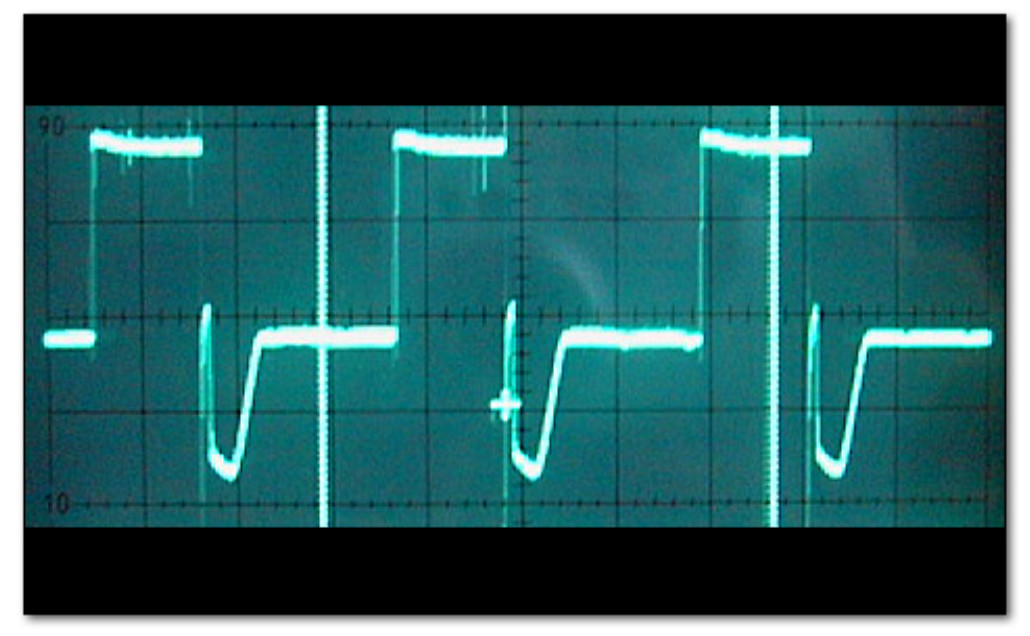
\includegraphics[width=\linewidth]{sensorless/scope.jpg}
}

\vspace{-1em}
\caption{\scriptsize Voltage characteristic at the motor terminals while a 
33\%~duty cycle PWM is applied~\cite{kerdels2008b}.}
\end{figure}
\end{column}
\begin{column}{0.28\textwidth}
\begin{figure}
{
\hspace{-0.5em}
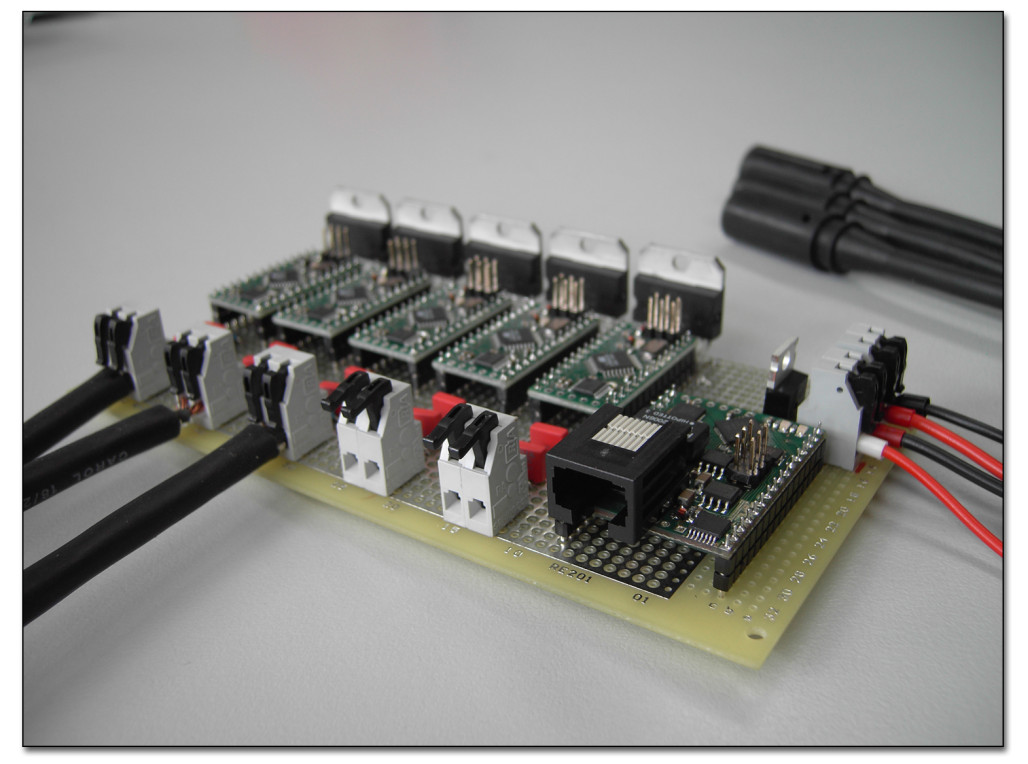
\includegraphics[width=0.98\linewidth]{sensorless/controller.jpg}
}

\vspace{-0.75em}
\caption{\scriptsize Electronic prototype to demonstrate the Back-EMF 
approach~\cite{kerdels2008b}.}
\end{figure}
\end{column}
\begin{column}{0.28\textwidth}
\begin{figure}
{
\hspace{-0.5em}
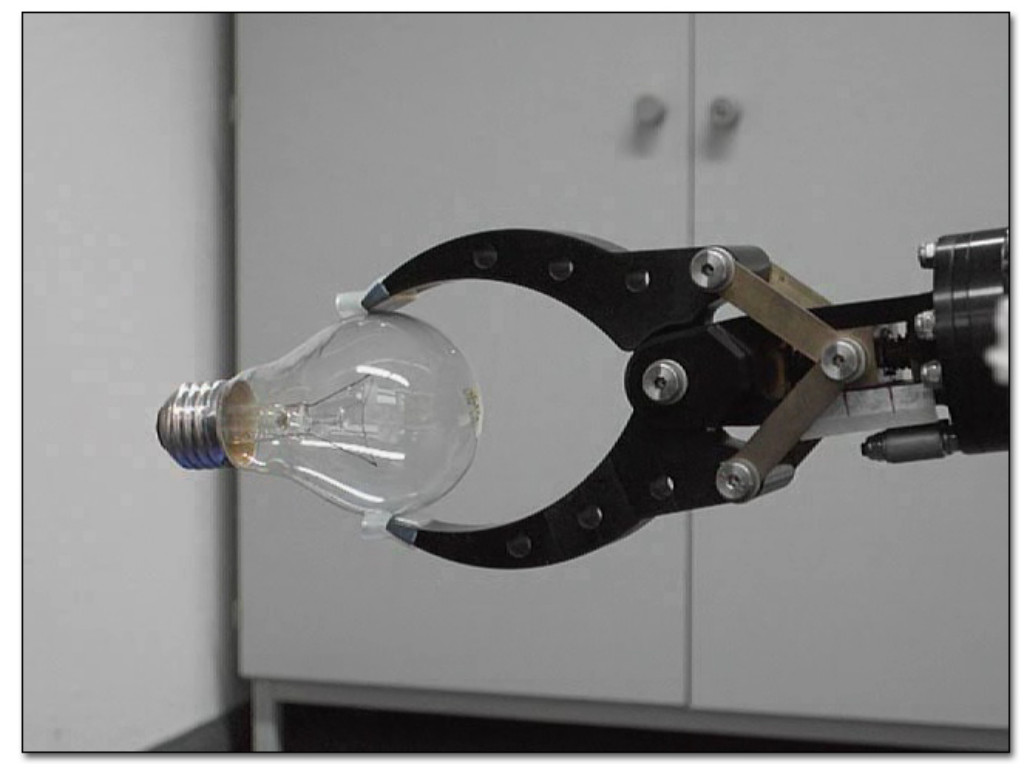
\includegraphics[width=0.98\linewidth]{sensorless/bulb.jpg}
}

\vspace{-0.75em}
\caption{\scriptsize Illustrating the sensitivity achievable with back EMF force 
control~\cite{kerdels2008b}.}
\end{figure}
\end{column}
\end{columns}	




%\vspace{1em}

\begin{center}
\rule{2cm}{0.4pt}\\[0.5em]
\end{center}

\fc{kerdels2008b}{publications/2008-02/2008-02}

\end{frame}
